%=============================================================================
% ACADEMIC CV — JOAQUIN LEAL ENCISO
% PhD / Research Applications
% Max: 2 pages | Engine: pdfLaTeX
%=============================================================================

\documentclass[11pt,a4paper]{article}

% -----------------------------------------------------------------------------
% Geometry
% -----------------------------------------------------------------------------
\usepackage[
top=0.6in,
bottom=0.6in,
left=0.7in,
right=0.7in
]{geometry}

% -----------------------------------------------------------------------------
% Fonts
% -----------------------------------------------------------------------------
\usepackage[T1]{fontenc}
\usepackage[utf8]{inputenc}
\usepackage{mathptmx}
\usepackage[scaled=0.92]{helvet}
\usepackage{courier}

% -----------------------------------------------------------------------------
% Packages
% -----------------------------------------------------------------------------
\usepackage[dvipsnames]{xcolor}
\usepackage{titlesec}
\usepackage{enumitem}
\usepackage{hyperref}
\usepackage{fancyhdr}
\usepackage{tabularx}
\usepackage{lastpage}
\usepackage{microtype}
\usepackage{graphicx}

% -----------------------------------------------------------------------------
% Colors
% -----------------------------------------------------------------------------
\definecolor{HeaderBlue}{HTML}{1A3C6E}
\definecolor{AccentGray}{HTML}{4A4A4A}
\definecolor{RULECOLOR}{HTML}{1A3C6E}
\definecolor{PhotoBorder}{HTML}{CCCCCC}

% -----------------------------------------------------------------------------
% PDF Metadata / Hyperlinks
% -----------------------------------------------------------------------------
\hypersetup{
	colorlinks=true,
	urlcolor=HeaderBlue,
	linkcolor=HeaderBlue,
	pdfauthor={Joaquin Leal Enciso},
	pdftitle={Joaquin Leal Enciso - Curriculum Vitae},
	pdfsubject={Academic Curriculum Vitae},
	pdfkeywords={
		Operations Research,
		Transportation Systems,
		Logistics,
		Mathematical Optimization,
		Electric Mobility
	}
}

% -----------------------------------------------------------------------------
% Section Formatting
% -----------------------------------------------------------------------------
\titleformat{\section}
{\large\bfseries\sffamily\color{HeaderBlue}\uppercase}
{}{0em}{}
[\vspace{-0.6em}{\color{RULECOLOR}\rule{\linewidth}{0.8pt}}]

\titleformat{\subsection}
{\normalsize\bfseries\sffamily\color{HeaderBlue}}
{}{0em}{}

\titleformat{\subsubsection}
{\normalsize\bfseries}
{}{0em}{}

\titlespacing*{\section}{0pt}{0.75em}{0.4em}

% -----------------------------------------------------------------------------
% Header / Footer
% -----------------------------------------------------------------------------
\pagestyle{fancy}
\fancyhf{}
\renewcommand{\headrulewidth}{0pt}

\fancyfoot[C]{
	\small\color{AccentGray}
	Page \thepage\ of \pageref{LastPage}
}

% -----------------------------------------------------------------------------
% Lists
% -----------------------------------------------------------------------------
\setlist[itemize]{
	leftmargin=1.2em,
	itemsep=1pt,
	parsep=0pt,
	topsep=2pt,
	label=\textbullet
}

% -----------------------------------------------------------------------------
% Custom Commands
% -----------------------------------------------------------------------------

% Organization | Location
% Position / Degree | Dates
\newcommand{\cventry}[4]{%
	\noindent
	\textbf{#1}\hfill\textit{#2}\\
	\textit{#3}\hfill{#4}
	\par\vspace{1pt}
}

% Simple line with right-aligned year/date
\newcommand{\cvline}[2]{%
	\noindent
	{#1}\hfill\textit{#2}
	\par\vspace{1pt}
}

% Photo placeholder
\newcommand{\photoplaceholder}{%
	\fcolorbox{PhotoBorder}{white}{%
		\parbox[c][3.2cm][c]{2.4cm}{%
			\centering
			\small
			\color{AccentGray}
			Your\\Photo\\Here
		}%
	}%
}

% -----------------------------------------------------------------------------
% General Spacing
% -----------------------------------------------------------------------------
\setlength{\parindent}{0pt}
\setlength{\parskip}{0pt}

%=============================================================================
\begin{document}
	
	%=============================================================================
	% HEADER
	%=============================================================================
	
	\noindent
	\begin{minipage}[c]{0.72\textwidth}
		
		{\LARGE
			\bfseries
			\sffamily
			\color{HeaderBlue}
			JOAQUIN LEAL ENCISO
		}\\[7pt]
		
		{\small
			
			Beijing, China\\[3pt]
			
			\href{mailto:joaquinleal6@buaa.edu.cn}
			{joaquinleal6@buaa.edu.cn}
			\enspace$\cdot$\enspace
			\href{https://jlab-eng.github.io}
			{jlab-eng.github.io}
			\enspace$\cdot$\enspace
			\href{https://github.com/jlab-eng}
			{github.com/jlab-eng}
			\\[3pt]
			
			\href{https://linkedin.com/in/joaquinleal}
			{LinkedIn}
			\enspace$\cdot$\enspace
			\href{https://orcid.org/0000-0001-9826-8715}
			{ORCID: 0000-0001-9826-8715}
			
		}
		
	\end{minipage}%
	\hfill
	\begin{minipage}[c]{0.24\textwidth}
		
		\raggedleft
		
		% Photo file must be in the same folder as this .tex file.
		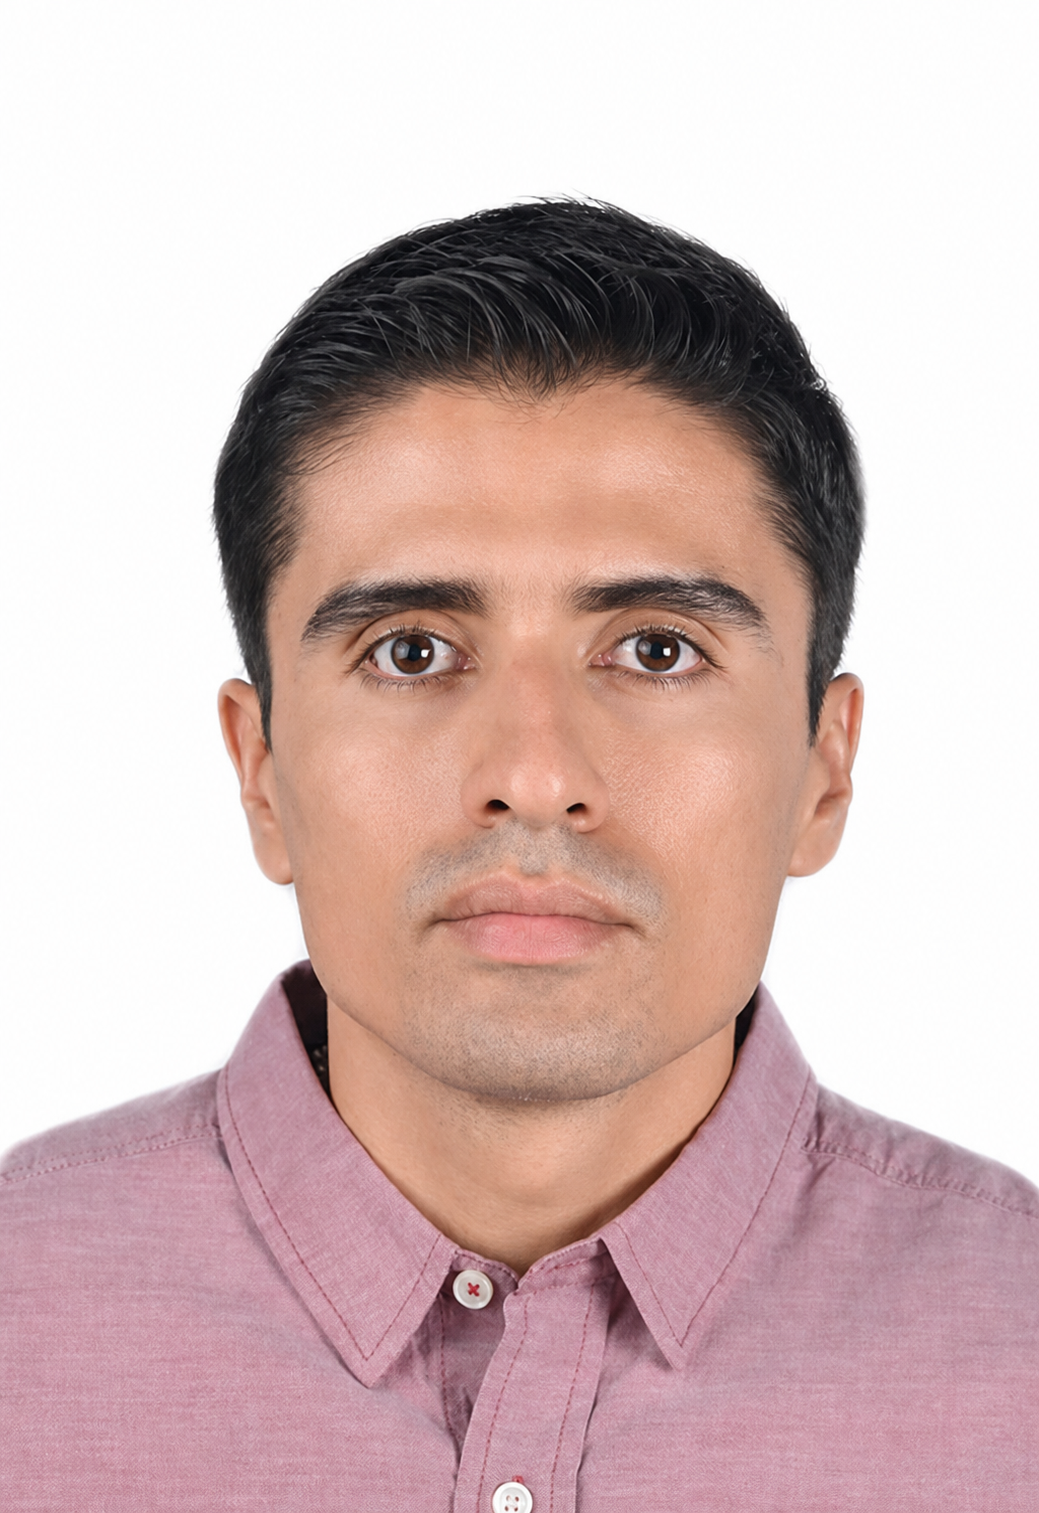
\includegraphics[
		width=2.4cm,
		height=3.2cm,
		keepaspectratio
		]{FOTO}
		
	\end{minipage}
	
	\vspace{0.3em}
	
	{\color{RULECOLOR}\rule{\linewidth}{0.8pt}}
	
	\vspace{-0.2em}
	
	
	%=============================================================================
	% RESEARCH INTERESTS
	%=============================================================================
	
	\section{Research Interests}
	
	Operations Research \& Decision Analysis
	\enspace$\cdot$\enspace
	Intelligent Transportation \& Smart Mobility
	\enspace$\cdot$\enspace
	Logistics, Supply Chain \& Resource Scheduling
	\enspace$\cdot$\enspace
	Machine Learning \& Operations Research
	
	
	%=============================================================================
	% EDUCATION
	%=============================================================================
	
	\section{Education}
	
	\cventry
	{Beihang University (BUAA)}
	{Beijing, China}
	{M.S. in Management Science and Engineering}
	{Sept 2024 -- Jun 2027}
	
	\begin{itemize}
		
		\item Thesis:
		``Optimization of Charging Scheduling for Battery Electric Buses (BEBs)
		Considering SoC-Dependent Charging Power.''
		Advisor: Prof.\ WANG Heixin.
		
		\item GPA: 3.68/4.00.
		Relevant coursework:
		Operations Research,
		Supply Chain Management,
		Macroeconomics and
		Microeconomics.
		
		
	\end{itemize}
	
	\vspace{4pt}
	
	\cventry
	{Industrial University of Santander}
	{Bucaramanga, Colombia}
	{B.Eng. in Mechanical Engineering}
	{Sept 2011 -- Jun 2016}
	
	\begin{itemize}
		
		\item Relevant coursework:
		Programming,
		Finite Element Analysis,
		and Economic Engineering.
		
	\end{itemize}
	
	
	%=============================================================================
	% RESEARCH EXPERIENCE
	%=============================================================================
	
	\section{Research Experience}
	
	\cventry
	{Beihang University}
	{Beijing, China}
	{Graduate Research Student}
	{Sept 2025 -- Present}
	
	\begin{itemize}
		
		\item Developed a
		\textbf{Mixed-Integer Linear Programming (MILP)}
		model for battery-electric bus charging and scheduling
		to minimize energy and operational costs under realistic
		fleet and infrastructure constraints.
		
		\item Implemented an optimization framework
		in \textbf{Python} using \textbf{Gurobi Optimizer}
		on a real-world battery-electric bus fleet case study
		a major BRT system in Bogotá, Colombia.
		
		\item Conducted a systematic review of more than 40 studies,
		identifying research gaps related to
		SoC-dependent charging-power modeling,
		electricity tariffs,
		and operational constraints.
		
	\end{itemize}
	
	\vspace{4pt}
	
	\cventry
	{Energy Lab}
	{Bucaramanga, Colombia}
	{Undergraduate Research Assistant}
	{2016}
	
	\begin{itemize}
		
		\item Performed finite element analysis (FEA)
		to characterize the mechanical behavior and structural integrity
		of Fiberspar composite pipes for crude-oil transportation
		applications in Colombia.
		
		\item Contributed to the mechanical characterization of a
		composite pipe technology newly introduced into the Colombian
		oil-transportation sector.
		
	\end{itemize}
	
	
	%=============================================================================
	% PUBLICATIONS
	%=============================================================================
	
	\section{Publications}
	
	\begin{itemize}
		
		\item
		\textbf{González-Estrada, O. A., Leal Enciso, J.,
			\& Reyes-Herrera, J. D.}
		(2016).
		``Structural integrity analysis of composite pipes
		for the transport of crude oil by finite elements.''
		\textit{UIS Ingenierías},
		\textit{15}(2), 105--106.
		DOI:
		\href
		{https://doi.org/10.18273/revuin.v15n2-2016009}
		{10.18273/revuin.v15n2-2016009}
		
	\end{itemize}
	
	
	%=============================================================================
	% TECHNICAL SKILLS
	%=============================================================================
	\newpage
	\section{Technical Skills}
	
	\begin{tabularx}{\linewidth}{@{}l X@{}}
		
		\textbf{Programming:}
		&
		Python, \LaTeX
		\\
		
		\textbf{Optimization:}
		&
		Gurobi Optimizer,
		Mixed-Integer Linear Programming (MILP),
		Mathematical Programming,
		Scheduling
		\\
		
		\textbf{AI \& Data-Driven Methods:}
		&
		AI-Assisted Decision-Making
		\\
		
		\textbf{Analysis:}
		&
		Sensitivity Analysis,
		Decision Analysis,
		Optimization Modeling
		\\
		
		\textbf{Software:}
		&
		VS Code,
		Jupyter,
		Plant Simulation
		\\
		
		\textbf{Languages:}
		&
		Spanish (Native),
		English (TOEFL),
		Mandarin Chinese (HSK 4)
		
	\end{tabularx}
	
	%=============================================================================
	% PAGE 2
	%=============================================================================
	

	
	
	%=============================================================================
	% PROFESSIONAL EXPERIENCE
	%=============================================================================
	
	\section{Professional Experience}
	
	\cventry
	{Wärtsilä}
	{Bogotá, Colombia}
	{Spare Parts Coordinator}
	{Aug 2023 -- Sept 2024}
	
	\begin{itemize}
		
		\item Coordinated quotations,
		order processing,
		and international logistics
		for maritime spare parts and critical engine components.
		
		\item Served as the coordination link between customers
		and internal departments including
		Field Service,
		Supply Chain,
		and Finance,
		supporting the resolution of technical and commercial
		non-conformities.
		
		\item Monitored response times and supply-chain flows
		to support service quality and timely delivery
		of critical vessel-engine components.
		
	\end{itemize}
	
	\vspace{4pt}
	
	\cventry
	{Contransmagdalena -- Regional Transport Company}
	{Bucaramanga, Colombia}
	{Maintenance Mechanical Engineer}
	{Feb 2018 -- Aug 2021}
	
	\begin{itemize}
		
		\item Developed a maintenance program for a fleet of diesel buses,
		supporting compliance with safety and service-level requirements.
		
		\item Organized and digitized technical vehicle records,
		improving data accessibility and maintenance-information management.
		
		\item Supported transportation-route and scheduling planning
		based on passenger demand,
		contributing to fleet utilization and service reliability.
		
	\end{itemize}
	
	
	%=============================================================================
	% AWARDS & HONORS
	%=============================================================================
	
	\section{Awards \& Honors}
	
	\cvline
	{\textbf{Master's Degree Full Scholarship},
		Chinese Scholarship Council}
	{2024}
	
	
	%=============================================================================
	% ADDITIONAL TRAINING
	%=============================================================================
	
	\section{Additional Training}
	
	\cvline
	{\textbf{Smart Cities Summer Course},
		Zhejiang University}
	{2025}
	
	\vspace{1pt}
	
	\noindent
	\hspace{0.5em}
	\small
	Focus areas:
	Smart Mobility,
	Urban Planning,
	and Sustainable Cities.
	\normalsize
	
	\vspace{5pt}
	
	\cvline
	{\textbf{Supply Chain Logistics},
		Rutgers University (Coursera)}
	{2024}
	
	\vspace{3pt}
	
	\cvline
	{\textbf{Python for Everybody},
		University of Michigan (Coursera)}
	{2024}
	
	
	%=============================================================================
	% END
	%=============================================================================
	
\end{document}